
所有构建流程都以相同的方式工作。从顶层列表文件开始,向下导航到项目源树。图12.4显示了参与构建的项目文件。括号中的数字表示CMake脚本执行的顺序:

\begin{center}
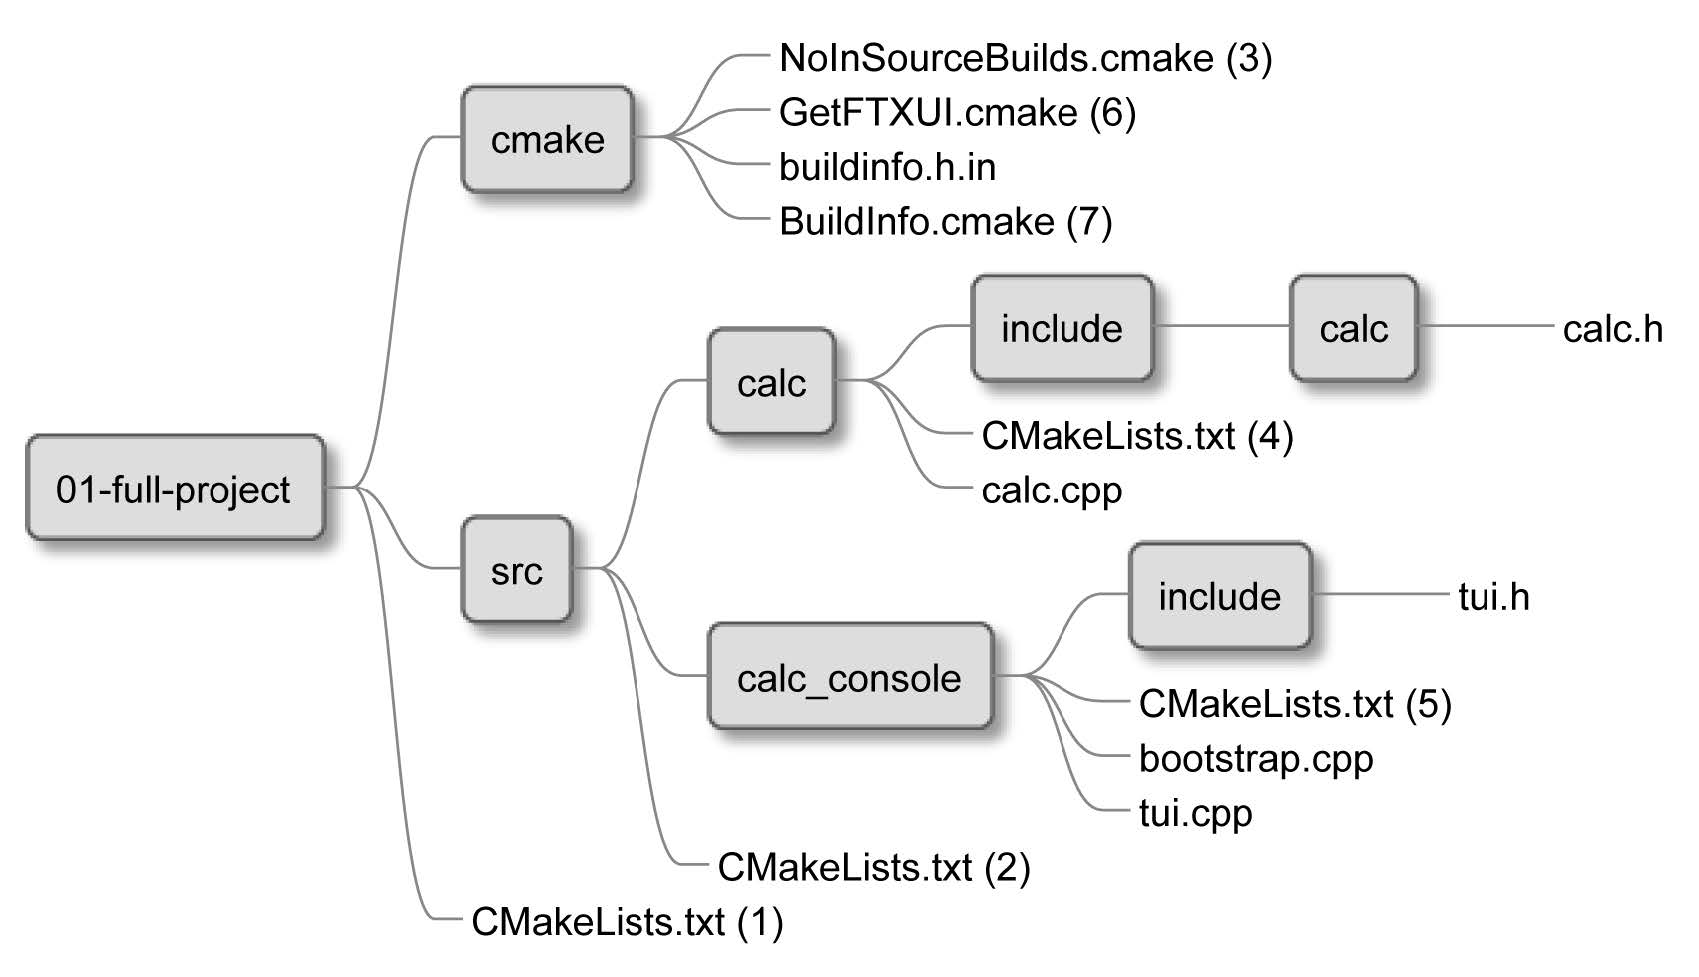
\includegraphics[width=0.6\textwidth]{content/3/chapter12/images/4.jpg}\\
图12.4 构建阶段使用的文件
\end{center}

顶层列表文件将配置项目,并加载嵌套元素:

\begin{lstlisting}[style=styleCMake]
# chapter-12/01-full-project/CMakeLists.txt

cmake_minimum_required(VERSION 3.20.0)
project(Calc VERSION 1.0.0 LANGUAGES CXX)
list(APPEND CMAKE_MODULE_PATH "${CMAKE_SOURCE_DIR}/cmake")

include(NoInSourceBuilds)

add_subdirectory(src bin)
add_subdirectory(test)

include(Install)
\end{lstlisting}

首先提供关键的项目细节,并添加到CMake实用程序模块的路径(项目中的CMake目录)。然后禁用源内构建(通过自定义模块),并包含两个关键目录:

\begin{itemize}
\item 
src,包含项目源(构建树中命名为bin)

\item 
test,包含所有测试实用程序
\end{itemize}

最后,将包含另一个模块,该模块将设置项目的安装。来看一看NoInSourceBuilds模块,了解它是如何工作的:

\begin{lstlisting}[style=styleCMake]
# chapter-12/01-full-project/cmake/NoInSourceBuilds.cmake

if(PROJECT_SOURCE_DIR STREQUAL PROJECT_BINARY_DIR)
	message(FATAL_ERROR
		"\n"
		"In-source builds are not allowed.\n"
		"Instead, provide a path to build tree like so:\n"
		"cmake -B <destination>\n"
		"\n"
		"To remove files you accidentally created execute:\n"
		"rm -rf CMakeFiles CMakeCache.txt\n"
	)
endif()
\end{lstlisting}

这里没有什么奇怪的——只是检查用户是否提供了一个目标目录作为cmake命令的参数来存储生成的文件,必须是与项目源树不同的路径。若不是这样,会通知用户如何提供,以及在错误发生后如何清理存储库。

顶层列表文件然后包含src子目录,指示CMake读取其中的列表文件:

\begin{lstlisting}[style=styleCMake]
# chapter-12/01-full-project/src/CMakeLists.txt

add_subdirectory(calc)
add_subdirectory(calc_console)
\end{lstlisting}

这个文件非常微妙——只是进入嵌套目录,执行其中的列表文件。让我们跟随calc库的列表文件——有点复杂,所以只讨论其中一部分。

\subsubsubsection{12.4.1\hspace{0.2cm}构建Calc库}

calc的列表文件包含一些测试配置,但现在将关注构建;其余的将在测试和程序分析部分讨论:

\begin{lstlisting}[style=styleCMake]
# chapter-12/01-full-project/src/calc/CMakeLists.txt (fragment)

add_library(calc_obj OBJECT calc.cpp)
target_include_directories(calc_obj INTERFACE
	"$<BUILD_INTERFACE:${CMAKE_CURRENT_SOURCE_DIR}/include>"
	"$<INSTALL_INTERFACE:${CMAKE_INSTALL_INCLUDEDIR}>"
)
set_target_properties(calc_obj PROPERTIES
	PUBLIC_HEADER src/calc/include/calc/calc.h
	POSITION_INDEPENDENT_CODE 1
)
add_library(calc_shared SHARED)
target_link_libraries(calc_shared calc_obj)
add_library(calc_static STATIC)
target_link_libraries(calc_static calc_obj)

# ... testing and program analysis modules
# ... documentation generation
\end{lstlisting}

声明三个目标:

\begin{itemize}
\item 
编译calc.cpp实现文件的对象库,并通过PUBLIC\_HEADER属性引用calc.h头文件,该属性可以在配置的include目录中找到(由于生成器表达式为特定模式提供了适当的路径——构建或安装)。通过使用这个库,避免了对其他目标的重复编译,还要启用POSITION\_INDEPENDENT\_CODE,以便动态库可以使用生成的目标文件。

\item 
calc\_shared,依赖于calc\_obj的动态库。

\item 
calc\_static,依赖于calc\_obj的静态库。
\end{itemize}

这里将添加calc库的C++代码:

\begin{lstlisting}[style=styleCXX]
// chapter-12/01-full-project/src/calc/include/calc/calc.h

#pragma once

namespace Calc {
	int Sum(int a, int b);
	int Multiply(int a, int b);
} // namespace Calc
\end{lstlisting}

这段代码非常基础:声明了两个包含在Calc命名空间中的全局函数(C++命名空间在库中非常有用,有助于避免名称冲突)。

实现文件也非常简单:

\begin{lstlisting}[style=styleCXX]
// chapter-12/01-full-project/src/calc/calc.cpp

namespace Calc {
int Sum(int a, int b) {
	return a + b;
}

int Multiply(int a, int b) {
	return a * b;
}
} // namespace Calc
\end{lstlisting}

这结束了src/calc目录中文件的解释。接下来是src/calc\_console,并使用这个库构建控制台计算器的可执行文件。

\subsubsubsection{12.4.2\hspace{0.2cm}构建Calc终端可执行文件}

calc\_console的源目录包含几个文件:一个列表文件、两个实现文件(业务代码和一个引导程序)和一个头文件。列表文件如下所示:

\begin{lstlisting}[style=styleCMake]
chapter-12/01-full-project/src/calc_console/CMakeLists.txt (fragment)
include(GetFTXUI)
add_library(calc_console_static STATIC tui.cpp)
target_include_directories(calc_console_static PUBLIC
	include)
target_precompile_headers(calc_console_static PUBLIC
	<string>)
target_link_libraries(calc_console_static PUBLIC
	calc_shared
	ftxui::screen ftxui::dom ftxui::component)
include(BuildInfo)
BuildInfo(calc_console_static)
# … testing and program analysis modules
# ... documentation generation

add_executable(calc_console bootstrap.cpp)
target_link_libraries(calc_console calc_console_static)
\end{lstlisting}

列表文件看起来很多,但作为有经验的CMake用户,可以很容易地理清里面发生的事情:

\begin{itemize}
\item 
包含CMake模块来获取FTXUI依赖

\item 
声明calc\_console\_static目标,该目标包含业务代码,但不包含main()函数,以允许GTest定义自己的入口点。

\item 
添加头文件的预编译——只是添加一个标准的字符串头文件来证明这一点,但是对于较大的项目,可以添加更多的头文件(包括属于项目的头文件)。

\item 
将业务代码与calc\_shared库和FTXUI库链接起来。

\item 
添加要在这个目标上执行的所有操作:生成构建信息、测试、程序分析和文档。

\item 
添加并链接calc\_console引导可执行文件,并提供了入口点。
\end{itemize}

同样,这里把测试和文档的讨论推迟到本章的后续部分。来看看依赖管理和构建信息生成。

注意,我们更喜欢使用实用程序模块,而不是查找模块来引入FTXUI。这是因为该依赖项不太可能已经存在于系统中。而不是希望找到它,我们将获取并安装它:

\begin{lstlisting}[style=styleCMake]
# chapter-12/01-full-project/cmake/GetFTXUI.cmake

include(FetchContent)
FetchContent_Declare(
	FTXTUI
	GIT_REPOSITORY https://github.com/ArthurSonzogni/FTXUI.git
	GIT_TAG v0.11
)
option(FTXUI_ENABLE_INSTALL "" OFF)
option(FTXUI_BUILD_EXAMPLES "" OFF)
option(FTXUI_BUILD_DOCS "" OFF)
FetchContent_MakeAvailable(FTXTUI)
\end{lstlisting}

使用推荐的FetchContent方法,第7章有详细介绍,唯一不同的添加是对option()指令的调用。其可以跳过FTXUI构建的冗长步骤,并将其安装配置从该项目的安装中分离出来。对于GTest依赖关系也需要同样的操作。option()指令在扩展阅读部分中有引用。

calc\_command的列表文件还包含一个与构建相关的自定义实用程序模块:BuildInfo。我们将使用它来记录三个可以在可执行文件中显示的值:

\begin{itemize}
\item 
当前Git提交的SHA

\item 
构建的时间戳

\item 
顶层列表文件中指定的项目版本
\end{itemize}

在第5章中,可以使用CMake来捕获一些构建时的值,并通过模板文件将其提供给C++代码——例如,使用C++结构体:

\begin{lstlisting}[style=styleCXX]
// chapter-12/01-full-project/cmake/buildinfo.h.in

struct BuildInfo {
	static inline const std::string CommitSHA =
		"@COMMIT_SHA@";
	static inline const std::string Timestamp =
		"@TIMESTAMP@";
	static inline const
	std::string Version = "@PROJECT_VERSION@";
};
\end{lstlisting}

为了在配置阶段填充该结构,可以使用以下代码:

\begin{lstlisting}[style=styleCMake]
# chapter-12/01-full-project/cmake/BuildInfo.cmake

set(BUILDINFO_TEMPLATE_DIR ${CMAKE_CURRENT_LIST_DIR})
set(DESTINATION "${CMAKE_CURRENT_BINARY_DIR}/buildinfo")

string(TIMESTAMP TIMESTAMP)
find_program(GIT_PATH git REQUIRED)
execute_process(COMMAND
	${GIT_PATH} log --pretty=format:'%h' -n 1
	OUTPUT_VARIABLE COMMIT_SHA)

configure_file(
	"${BUILDINFO_TEMPLATE_DIR}/buildinfo.h.in"
	"${DESTINATION}/buildinfo.h" @ONLY
)

function(BuildInfo target)
	target_include_directories(${target} PRIVATE
		${DESTINATION})
endfunction()
\end{lstlisting}

包含该模块将设置包含所需要的信息的变量,然后使用configure\_file()来生成buildinfo.h。剩下的就是调用BuildInfo函数,并添加生成文件的目录,以包含所需目标的目录。然后,可以与多个不同的使用者共享该文件,并且可能需要在列表文件的顶部添加include\_guard(GLOBAL),以避免对每个目标都运行git命令。

深入研究控制台计算器的实现之前,不应该过分担心tui.cpp文件的复杂性。要完全理解它,只需要对FXTUI库有一定的了解——我们不想太深入。相反,让我们关注突出显示的行:

\begin{lstlisting}[style=styleCXX]
// chapter-12/01-full-project/src/calc_console/tui.cpp

#include "tui.h"
#include <ftxui/dom/elements.hpp>
#include "buildinfo.h" // 突出显示的行
#include "calc/calc.h" // 突出显示的行

using namespace ftxui;
using namespace std;

string a{"12"}, b{"90"};
auto input_a = Input(&a, "");
auto input_b = Input(&b, "");
auto component = Container::Vertical({input_a, input_b});

Component getTui() {
	return Renderer(component, [&] {
		auto sum = Calc::Sum(stoi(a), stoi(b)); // 突出显示的行
		return vbox({
			text("CalcConsole " + BuildInfo::Version), // 突出显示的行
			text("Built: " + BuildInfo::Timestamp), // 突出显示的行
			text("SHA: " + BuildInfo::CommitSHA), // 突出显示的行
			separator(),
			input_a->Render(),
			input_b->Render(),
			separator(),
			text("Sum: " + to_string(sum)), // 突出显示的行
			}) |
		border;
	});
}
\end{lstlisting}

这段代码提供了一个getTui()函数,返回一个ftxui::Component对象,该对象封装了一个带有标签、文本字段、分隔符和边框的交互式UI元素。若对它的详细工作原理感兴趣,可以在扩展阅读部分找到合适的参考资料。

更重要的是,了解一下include指令:其引用了用calc\_obj目标和BuildInfo模块提供的头文件。提供给Renderer类构造函数的lambda函数的第一行将调用库的Calc::Sum方法,并使用结果值打印带有Sum的标签(通过调用下面的text()函数)。

类似地,标签用于向用户显示在构建时,通过连续三次调用text()来收集BuildInfo::values 。

这个方法在相关的头文件中有声明:

\begin{lstlisting}[style=styleCXX]
// chapter-12/01-full-project/src/calc_console/include/tui.h

#include <ftxui/component/component.hpp>
ftxui::Component getTui();
\end{lstlisting}

然后,被calc\_console目标使用:

\begin{lstlisting}[style=styleCXX]
// chapter-12/01-full-project/src/calc_console/bootstrap.cpp

#include <ftxui/component/screen_interactive.hpp>
#include "tui.h"

int main(int argc, char** argv) {
	ftxui::ScreenInteractive::FitComponent().Loop(getTui());
}
\end{lstlisting}

这段简短的代码利用ftxui创建一个交互式控制台屏幕,该屏幕接受getTui()返回的Component对象,使其对用户可见,并在循环中收集键盘事件,创建一个界面,如图12.1所示。同样,理解这一点并不真正重要,因为ftxui的主要目的是为我们提供一个外部依赖项,重要的是其可以使用它来练习CMake技术。

已经介绍了src目录中的所有文件。接下来,来看看测试和分析程序。





